\def \sectionauthors {Samuel Bleiner}
\subsection{Anforderungen}
\lipsum[1-5]
\subsection{Vorstudie}
\lipsum[1-5]

\subsection{Bildverarbeitung}

\subsubsection{Einleitung}
Die Bildverarbeitung ist ein zentrales Thema in dieser Applikation für Kennzeichenerkennung. 
Sie wird für die Zeichensegmentierung verwendet, sowie für die Vorbereitung von Bildern für 
andere Algorithmen. Im Folgenden werden die verwendeten Bildverarbeitungsfunktionen aufgelistet 
und deren Funktionsweise erläutert.

\subsubsection{Bilaterale Filterung}
Bilaterale Filterung ist eine Methode für eine kantenerhaltende Weichzeichnung eines Bildes.\\

Bei der Berechnung für den Farbwert des Ausgabepixels werden die benachbarten Pixel nicht nur 
mit ihrer Entfernung gewichtet, sondern auch mit ihrem eigenen Farbwert. Dadurch können einzelne 
farbliche Ausreißer herausgefiltert werden. Dies ist vor allem in der Bildverarbeitung wichtig, 
da dadurch die wichtigen Eigenschaften eines Bildes, wie zum Beispiel Kanten, erhalten bleiben 
und verarbeitet werden können, aber einzelne abweichende Pixel herausgefiltert werden wodurch 
unnötige Informationen entfernt werden.\\ 

\begin{figure}[htbp]
    \centering
    \begin{minipage}[t]{0.45\linewidth}
        \centering
        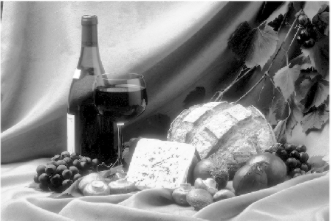
\includegraphics[width=\linewidth]{kennzeichenerkennung/vorBilateral.png}
        \caption{Vor Bilateraler Filterung}
        \label{vorBi}
    \end{minipage}
    \hfill
    \begin{minipage}[t]{0.45\linewidth}
        \centering
        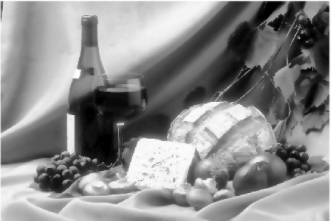
\includegraphics[width=\linewidth]{kennzeichenerkennung/nachBilateral.png}
        \caption{Nach Bilateraler Filterung}
        \label{nachBi}
    \end{minipage}
\end{figure}

In Abbildung \ref{vorBi} kann man ein Bild von verschieden Lebensmitteln sehen. Wenn man genau hinsieht 
erkennt man vor allem bei den Blättern im Hintergrund und beim Brot viele detailreiche Texturen. 
Diese Texturen haben keine wichtige Texturen und sind deswegen unnötig. Um die Bildverarbeitung zu 
vereinfachen wendet man deswegen die bilaterale Filterung auf dieses Bild an, um diese detailreichen 
Texturen zu vereinfachen. In Abbildung \ref{nachBi} sieht man das Bild nach der bilateralen Filterung. 
Wenn man hier dann wieder genauer auf die Blätter und das Brot sieht, erkennt man, dass die 
detailreichen Texturen weichgezeichnet wurden, aber die Kanten sind genauso gut erkennbar wie vor der Filterung.

\subsubsection{Thresholding}
Das Thresholding oder auch Schwellenwertverfahren wird in der Bildverarbeitung verwendet, um Bilder zu segmentieren. 
Aus einem Graubild kann dadurch ein Binäres Bild erzeugt werden.\\ 

Bei diesem Verfahren wird ein bestimmter Schwellwert (En.: Threshold) definiert, welcher mit den Grauwerten der einzelnen 
Pixel des Bildes verglichen wird. Wenn der Grauwert den Schwellwert überschreitet, wird dieser durch einen weißen Pixel 
ersetzt und wenn der Grauwert kleiner als der Schwellwert ist, wird dieser durch einen schwarzen Pixel ersetzt. 
Dadurch erhält man ein Bild welches nur noch zwei Farben hat, Schwarz und Weiß. Dies wird deswegen eingesetzt, 
da dadurch viele Bildverarbeitungsalgorithmen schneller arbeiten und die Effizienz gesteigert wird.\\

\begin{figure}[htbp]
    \centering
    \begin{minipage}[t]{0.45\linewidth}
        \centering
        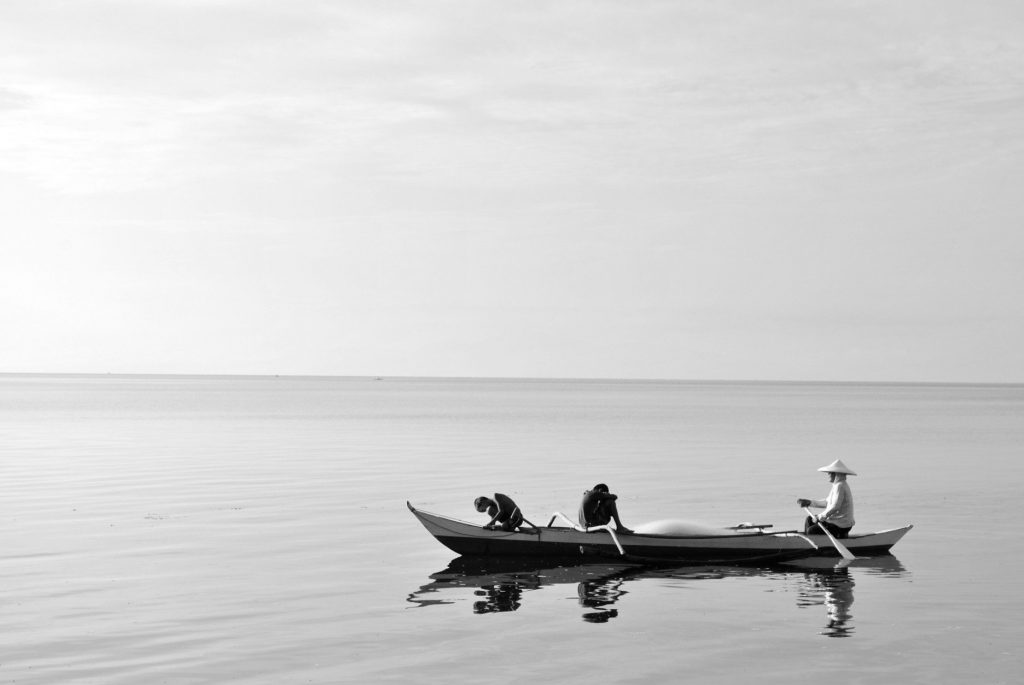
\includegraphics[width=\linewidth]{kennzeichenerkennung/graustufen.png}
        \caption{Graustufenbild}
        \label{graypic}
    \end{minipage}
    \hfill
    \begin{minipage}[t]{0.45\linewidth}
        \centering
        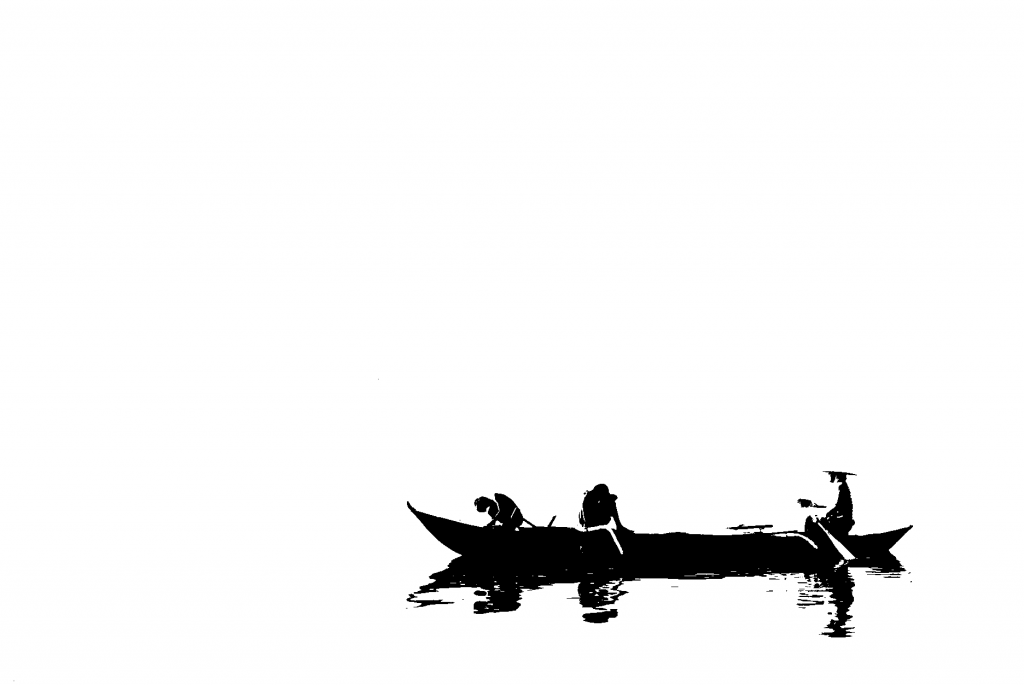
\includegraphics[width=\linewidth]{kennzeichenerkennung/binary.png}
        \caption{Binäres Bild nach Thresholding}
        \label{binarypic}
    \end{minipage}
\end{figure}

In Abbildung \ref{graypic} sieht man ein solches Graubild welches nur verschieden Graustufen aufweist. In Abbildung \ref{binarypic} sieht man das 
Bild nach dem Thresholding. Hier kann man nur noch das Boot mit den Menschen erkennen. Dies ist nicht nur für schnellere 
Bildverarbeitungsalgorithmen wichtig, sondern wird auch zur Objekterkennung in Bildern verwendet.\\

Um den Schwellwert zu bestimmen kann man diesen entweder variieren bis das gewünschte Ergebnis erscheint oder man 
verwendet Methoden, welche den Schwellwert automatisch bestimmen. Eine der bekanntesten Methoden zur Schwellwertbestimmung 
ist die Methode von Otsu\footnote{Benannt nach Nobuyuki Otsu}, welche mit dem Schwellenwert die Pixel in Vordergrund und Hintergrund unterteilt.

\subsubsection{Erosion}
Erosion ist eine Funktion der Bildverarbeitung und ist in die morphologische Bildverarbeitung einzuordnen. Diese beschäftigt 
sich primär mit der Verarbeitung von binären Bildern, welche man nach Thresholding erhält.\\

Erosion benötigt zwei Eingaben, das binäre Bild und einen Kernel. Der Kernel ist dabei die Angabe, nach welcher die Erosion 
durchgeführt wird. Der Kernel ist auch eine binäre Struktur, welche über jeden einzelnen Pixel des binären Bildes geschoben 
wird. Wenn der Kernel komplett mit dem binären Bild übereinstimmt, behält dieser Pixel seinen Wert und ansonsten wird er 
invertiert. Dabei muss jedoch darauf geachtet werden, dass die Polarität des binären Bildes und des Kernels übereinstimmt, 
da sonst die Erosion nicht richtig funktioniert. Als Resultat erhält man danach ein deutlicheres Bild bei welchem einzelne 
Pixelfehler herausgefiltert wurden und die Konturen besser erkennbar sind.\\

\begin{figure}[htbp]
    \centering
    \begin{minipage}[t]{0.45\linewidth}
        \centering
        
\includegraphics[width=\linewidth]{kennzeichenerkennung/kennBinary.png}
        \caption{Binäres Bild nach Thresholding}
        \label{kennbinpic}
    \end{minipage}
    \hfill
    \begin{minipage}[t]{0.45\linewidth}
        \centering
        
\includegraphics[width=\linewidth]{kennzeichenerkennung/kennErosion.png}
        \caption{Nach Erosion}
        \label{eropic}
    \end{minipage}
\end{figure}

In Abbildung \ref{kennbinpic} und \ref{eropic} sieht man die Anwendung der Erosion. Die Konturen der einzelnen Zeichen im Kennzeichen sind in Abbildung 
\ref{eropic} nach der Erosion deutlicher erkennbar als davor.

\subsubsection{Farbraum}
Der Farbraum eines Bildes enthält alle möglichen Farben eines Farbmodells. Das Farbmodell beschreibt dabei die Parameter, aus 
welchen die einzelnen Farben gebildet werden. Dies ist in der Bildverarbeitung relevant, da verschiedene Funktionen der 
Bildverarbeitung, unterschiedliche Farbräume verwenden und dieser deswegen korrekt eingestellt werden muss.\\

In dieser spezifischen Applikation werden die folgenden Farbräume verwendet:

\paragraph{RGB}\mbox{}\\
RGB ist einer der häufigsten und bekanntesten Farbräume. Er basiert auf den drei Grundfarben Rot, Grün und Blau und wird vor 
allem bei Bildschirmen und in der Fotografie genutzt. Die Farben setzen sich in diesem Modell aus dem jeweiligen Rot-, Grün- 
und Blauanteil der einzelnen Pixel zusammen.

\paragraph{Graustufen}\mbox{}\\
Bei einem Graustufen-Bild, zu sehen in Abbildung 3, hat jeder Pixel einen Wert von 0 bis 255. Diese Werte erstrecken sich also 
von Schwarz bis Weiß und dazwischen liegen verschiedene Grautöne. Dieser Farbraum wird in der Bildverarbeitung häufig verwendet, 
da Konturen einfacher erkennbar sind und es nur einen Parameter gibt, welcher verarbeitet werden muss, wodurch die Effizienz 
diverser Algorithmen gesteigert werden kann. Zudem wird dieser Farbraum auch oft in Verbindung mit Thresholding verwendet.

\paragraph{BGR}\mbox{}\\
Der BGR ist ein relativ unbekannter und wenig verwendeter Farbraum, da er sehr ähnlich zum RGB-Farbraum ist. Der einzige 
Unterschied zwischen diesen beiden liegt in der Anordnung der Parameter. Bei BGR sind die Parameter spiegelverkehrt zu RGB, 
das heißt es kommt zuerst der Blauanteil, dann der Grünanteil und zum Schluss der Rotanteil. Insgesamt ergibt dies für die 
einzelnen Pixel zwar die gleichen Farben, aber die Funktionen der Bildverarbeitung müssen trotzdem das Bild im passenden 
Farbraum erhalten. So verwendet zum Beispiel die Funktion „imread“ von OpenCV den BGR-Farbraum und die Funktion „im Show“ 
von Matplotlib verwendet den RGB-Farbraum. Wenn man diese Funktionen also nacheinander anwendet, muss dazwischen der Farbraum 
umgewandelt werden.

\subsubsection{Konturerkennung}
Die Konturerkennung ist eine wichtige Funktion in der Bildverarbeitung mit welcher Objekte in einem Bild gefunden werden können. 
In dieser Applikation wird sie für die Zeichensegmentierung eingesetzt.\\

Die Konturerkennung wird hauptsächlich bei binären Bildern verwendet. Eine Kontur kann dabei wie im Folgenden definiert werden. 
Man überprüft jeden einzelnen Pixel und sieht nach, ob ein benachbarter Pixel einen anderen Farbwert aufweist. Falls dies 
zutrifft muss der zu prüfende Pixel zu einer Kontur gehören. Wenn dies auf mehrere zusammenhängende Pixel zutrifft, bedeutet 
das, dass diese zusammen eine Kontur bilden.\\

Die Funktion „findcontours“ von OpenCV, welche in dieser Applikation verwendet wird, ist eine Funktion für Konturerkennung 
und kann weiße Objekte auf einem schwarzen Hintergrund erkennen. Sie basiert auf dem Algorithmus von Suzuki von 
1985\footnote{Topological structural analysis of digitized binary images by border following} und 
liefert eine Liste mit allen Konturen. Die Konturen werden in der Liste als ein Array von Koordinaten abgespeichert.

\subsection{Kennzeichenerkennungsprogramm}

\subsubsection{Einleitung}
Die Software ist der wichtigste und größte Teil der Kennzeichenerkennung. Sie erhält ein Bild, in welchem ein Auto mit 
einem Kennzeichen enthalten ist und liefert am Ende dieses Kennzeichen und sendet dieses dann automatisch an die Datenbank. 
Die Software kann entweder über Bildverarbeitung oder mit Machine Learning Modellen realisiert werden. Der erste Ansatz bei 
dieser Anwendung war mit klassischer Bildverarbeitung, welche aber nicht die gewünschte Genauigkeit erreicht hat, weswegen 
dann auf Machine Learning gewechselt wurde.

\subsubsection{Programmiersprache}
Die verwendete Programmiersprache für die Kennzeichenerkennung ist Python. Python ist eine höhere Programmiersprache, 
welche übersichtlich und leicht lesbar ist. Sie ist vor allem für Bildverarbeitung und Machine Learning Anwendungen gut geeignet, 
da es dafür hoch optimierte und effiziente Bibliotheken gibt wie zum Beispiel OpenCV, Numpy und Tensorflow. Dadurch ist Python 
für diese Anwendung besser geeignet als zum Beispiel C++. Dieses wäre zwar normalerweise effizienter, bietet aber weniger 
optimierte Bibliotheken in diesem Bereich, wodurch es hier weniger gut geeignet ist.

\subsubsection{Konzept}
Das Programm für die Kennzeichenerkennung basiert auf fünf Stufen. Die erste Stufe ist die Bildaufnahme, die zweite ist die 
Kennzeichenerfassung mittels Machine Learning, die dritte ist die Kennzeichensegmentierung mithilfe von Bildverarbeitung, 
die vierte ist die Zeichenerkennung mittels Machine Learning und die fünfte ist die Anbindung an die Datenbank.

\paragraph{Bildaufnahme}\mbox{}\\
Um ein Bild verarbeiten zu können und aus diesem ein Kennzeichen auslesen zu können, muss zuerst ein Bild vorliegen. 
Dieses wird über den RaspberryPi mit der RaspberryPi-Kamera aufgenommen. Um das Bild aufzunehmen, muss einfach ein Auslöser 
aktiviert werden und dann wird das Bild aufgenommen und im richtigen Ordner abgespeichert. Zuvor wird noch überprüft ob 
sich in diesem Ordner bereits ein Bild befindet und falls eines vorhanden ist wird es gelöscht. Dadurch werden mögliche Fehler 
durch mehrere Bilder verhindert.

\paragraph{Kennzeichenerfassung}\mbox{}\\
Die Kennzeichenerfassung hat die Aufgabe, das Kennzeichen im Eingabebild zu lokalisieren. Dies geschieht mittels Machine Learning 
mit dem Modul WPOD-NET von Sérgio Montazolli Silva und Cláudio Rosita Jung\footnote{License Plate Detection and Recognition in Unconstrained Scenarios}. Dieses verwendet zuerst das Modul YOLOv2 welches zur 
Echtzeitobjekterkennung verwendet werden kann und in dieser Anwendung zur Erkennung von Fahrzeugen verwendet wird. Danach werden 
die Koordinaten des Kennzeichens ermittelt und dieses aus dem Bild ausgeschnitten und abgespeichert.

\paragraph{Kennzeichensegmentierung}\mbox{}\\
Die Kennzeichensegmentierung hat das Ziel die einzelnen Zeichen im Kennzeichen zu separieren und so zu vorbereiten, dass die 
darauffolgende Zeichenerkennung damit arbeiten kann. Dazu wird das Bild mit dem Kennzeichen zuerst in Graustufen konvertiert, 
dann mit einem bilateralen Filter gefiltert, mit Thresholding in ein binäres Bild umgewandelt und anschließend mittels Erosion 
besser erkennbar gemacht. Danach werden im verarbeiteten Bild die Konturen gesucht, sortiert und anhand dieser die einzelnen Zeichen herausgefiltert.

\paragraph{Zeichenerkennung}\mbox{}\\
Die letzte Stufe der Kennzeichenerkennung ist die Zeichenerkennung. In dieser werden die einzelnen Zeichen erkannt und als Text 
abgespeichert. Dies funktioniert über eine eigenes Neuronales Netz basierend auf MobileNetV2\footnote{Neuronales Netz für Computer Vision}, welches mit einem Datensatz von 
über 35 000 Bildern auf die Erkennung von Zeichen aus Bildern trainiert wurde.

\paragraph{Anbindung an Datenbank}\mbox{}\\
Nachdem das Kennzeichen als Text abgespeichert wurde, muss diese Information in die Datenbank übergeben werden. Dazu wird die 
eigene API angewandt, welcher man diese Informationen übergeben muss und als Rückgabe die Information bekommt, ob sich das 
Fahrzeug nun innerhalb oder außerhalb des Parkplatzes befindet.

\subsubsection{Ablauf}

\begin{figure}[H]
    \centering
    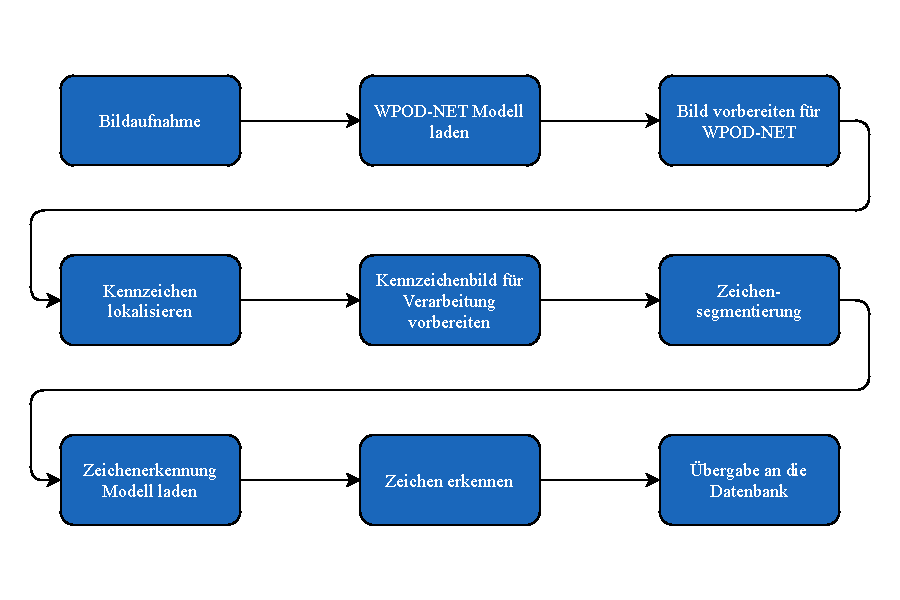
\includegraphics[width=0.9\linewidth]{kennzeichenerkennung/Programmablauf.pdf}
    \caption{Ablaufdiagramm der Kennzeichenerkennung}
\end{figure}

Im oberen Diagramm ist der Ablauf des Programms angegeben. Zuerst wird mit einem Button der Auslöser betätigt und damit das 
Foto aufgenommen. Dann wird das erste Machine Learning Modell für die Kennzeichenerkennung „WPOD-NET“\footnote{Machine Learning Modell für Kennzeichenerfassung} geladen. Bevor das 
Bild diesem Modell übergeben werden kann, muss es noch angepasst werden damit das Modell damit arbeiten kann. Danach kann 
damit das Kennzeichen im Bild lokalisiert werden. Im Anschluss wird dieses Kennzeichenbild mit mehreren Bildverarbeitungsalgorithmen 
verarbeitet, um dann die einzelnen Zeichen zu segmentieren. Danach kann dann das Modell für die Zeichenerkennung geladen 
werden und dieses dann auch angewendet werden, um das Ergebnis zu erhalten. Dieses Ergebnis wird dann noch mit einer API an die Datenbank übergeben.

\subsubsection{Verwendete Libraries}

\paragraph{Versionsübersicht der verwendeten Libraries}\mbox{}\\
Im Folgenden werden die verwendeten Versionen der benötigten Libraries aufgelistet, um das Programm zu starten. Dies wird noch einmal 
unterteilt in die Versionen, welche auf Windows 10 benötigt werden und jene auf Raspbian\footnote{Raspbian ist ein Unix-basiertes Betriebssystem für den Raspberry Pi}, da auf Raspbian manche Versionen noch 
nicht verfügbar sind, neuere und verbesserte Versionen verfügbar sind oder manche Versionen nur auf komplizierten Umwegen installierbar sind.

Windows:

\begin{itemize}
    \item h5py = 2.10.0
    \item imutils = 0.5.3
    \item Keras = 2.4.3
    \item matplotlib = 3.3.2
    \item notebook = 6.1.5
    \item numpy = 1.18.5
    \item opencv-python = 4.4.0.44
    \item scikit-learn = 0.23.2
    \item tensorflow = 2.3.1
    \item requests = 2.24.0
\end{itemize}

Raspbian:

\begin{itemize}
    \item h5py = 2.10.0
    \item imutils = 0.5.3
    \item Keras = 2.4.3
    \item matplotlib = 3.3.3
    \item notebook = 6.1.5
    \item numpy = 1.19.4
    \item opencv-python = 4.4.0.46
    \item scikit-learn = 0.24.0
    \item tensorflow = 2.4.0
    \item requests = 2.21.0
\end{itemize}

\paragraph{Jupyter Notebook}\mbox{}\\
Jupyter Notebook ist eine nützliche Erweiterung für Python, wenn es um den Bereich der Daten-Visualisierung und Machine Learning geht. 
Sie ist eine Unteranwendung des Open-Source Projektes „Project Jupyter“, welches von großen Partnern wie Microsoft und Google unterstützt 
und verwendet wird. Mit Jupyter Notebook ist es möglich in einer Web-Anwendung ein Live-Script abzuarbeiten und in Kombination mit Matplotlib 
die Daten visuell darzustellen, abzuspeichern und zu überwachen. Im Gegensatz zur direkten Darstellung in der Entwicklungsumgebung, wird 
der letzte Durchgang des Scripts, inklusive aller Bilder und Grafiken gespeichert. Zudem ist es auch hervorragend für das Training und 
die dazugehörende Überwachung von Machine Learning Modulen geeignet. Außerdem bietet Jupyter Notebook noch die Möglichkeit mehrere Scripts 
parallel abzuarbeiten und diese individuell zu überwachen. In dieser Applikation wird es für ein solches Training und für die anschauliche 
Visualisierung von Daten genutzt.\\

Die Installation von Jupyter Notebook ist simpel, da man es einfach über pip\footnote{Paketverwaltungsprogramm für Python} mit dem folgenden Befehl installieren kann:

\begin{listing}[H]
    \begin{minted}{bash}
    pip install notebook
    \end{minted}
    \caption{PIP Installation von Jupyter Notebook}
\end{listing}

Um das Jupyter Notebook aufzurufen muss im Terminal „jupyter notebook“ eingegeben werden und dann öffnet sich automatisch die Web-Applikation. 
Danach hat man Zugriff auf komplette Dateistruktur des eigenen Projektes und kann die einzelnen Python-Scripts starten. Dabei ist zu beachten, 
dass man keine gewöhnliche .py-Datei benötigt, sondern eine .ipynb-Datei benötigt, wozu man einfach eine Kopie des normalen Scripts erstellt und die Dateiendung ändert.

\paragraph{Numpy}\mbox{}\\
Numpy ist eine weit verbreitete Library für Python, welche sich mit der Berechnung und Verarbeitung von mehrdimensionalen Arrays beschäftigt. 
Damit können komplexe Berechnungen und Algorithmen oft effizienter verarbeitet werden, wobei aber beachtet werden muss, dass der Code an die 
mehrdimensionalen Arrays angepasst werden muss. Numpy selbst ist auch eine Voraussetzung für OpenCV, welches Numpy-Arrays verwendet, um Bilder zu verarbeiten. 
Dazu werden 3-dimensionale Arrays verwendet, wodurch die Verarbeitung dieser Bilder und die Bildverarbeitungsalgorithmen schneller sind. In dieser 
Applikation wird Numpy in Zusammenarbeit mit OpenCV verwendet und auch für die weitere Verarbeitung der Daten von OpenCV, um zum Beispiel die 
Koordinaten des Kennzeichens zu speichern.\\

Um Numpy zu installieren muss folgender Befehl in der Konsole eingegeben werden:

\begin{listing}[H]
    \begin{minted}{bash}
    pip install numpy
    \end{minted}
    \caption{PIP Installation von Numpy}
\end{listing}

\paragraph{OpenCV}\mbox{}\\
OpenCV ist die wichtigste und mächtigste Library die in dieser Applikation verwendet wird. Sie wurde ursprünglich in C++ geschrieben, 
aber es gibt auch eine Version in Python, welche in dieser Applikation verwendet wird. OpenCV ist eine freie Library für Bildverarbeitung, 
Computer Vision\footnote{Die Computergestütze Auswertung und Verarbeitung von Kamerabildern} und Machine Learning, welche von Intel gestartet wurde und mittlerweile die wichtigste und am weitesten verbreitete 
Library in diesem Bereich ist. Sie verwendet Numpy-Arrays, um für eine effiziente Verarbeitung von Bildern zu sorgen. Einige der wichtigsten 
Funktionen stellen die klassischen Bildverarbeitungsalgorithmen wie zum Beispiel Filterung und Farbraumanpassungen, die Verarbeitung und 
Auswertung von Kamerabildern und auch die Kompatibilität mit Deep-Learning\footnote{Machine Learning Methode welche Neuronale Netze nutzt} dar. In dieser Applikation wird OpenCV für diverse 
Bildverarbeitungsalgorithmen, die Zusammenarbeit mit Machine Learning Modulen, die Verarbeitung eines Kamerabildes und das allgemeine Arbeiten mit Bildern verwendet.\\

Die Installation von OpenCV ist dabei etwas komplizierter als bei anderen Librarys.\\

Windows:\\

Unter Windows ist die Installation vergleichbar mit anderen Libraries, es muss einfach der folgende Befehl in der Konsole eingegeben werden:

\begin{listing}[H]
    \begin{minted}{bash}
    pip install opencv-python
    \end{minted}
    \caption{PIP Installation von OpenCV}
\end{listing}

Raspbian:\\

Auf dem Raspberry Pi gestaltet sich die Installation von OpenCV um einiges schwieriger, da die Installation nicht über pip gemacht werden kann, 
sondern es manuell kompiliert werden muss.\\

Als erstes werden alle Tools und Bibliotheken installiert, welche für OpenCV benötigt werden. Dazu verwendet man folgenden Befehl im Terminal:

\begin{listing}[H]
    \begin{minted}{bash}
    $ sudo apt-get install build-essential git cmake pkg-config libjpeg8-dev libtiff4-dev libjasper-dev libpng12-dev libavcodec-dev libavformat-dev libswscale-dev libv4l-dev libgtk2.0-dev libatlas-base-dev gfortran
    \end{minted}
    \caption{Installation benötigter Tools und Bibliotheken für OpenCV}
\end{listing}

Danach kann man mit dem nächsten Befehl OpenCV von einem GitHub-Repository klonen:

\begin{listing}[H]
    \begin{minted}{bash}
    $ sudo apt-get install build-essential git cmake pkg-config libjpeg8-dev libtiff4-dev libjasper-dev libpng12-dev libavcodec-dev libavformat-dev libswscale-dev libv4l-dev libgtk2.0-dev libatlas-base-dev gfortran
    \end{minted}
    \caption{Klonen von OpenCV von GitHub}
\end{listing}

Im nächsten Schritt wird OpenCV mit den folgenden Befehlen kompiliert:

\begin{listing}[H]
    \begin{minted}{bash}
    cd ~/opencv && mkdir build && cd build

    cmake -D CMAKE_BUILD_TYPE=RELEASE \
    -D CMAKE_INSTALL_PREFIX=/usr/local \
    -D INSTALL_PYTHON_EXAMPLES=ON \
    -D INSTALL_C_EXAMPLES=ON \
    -D OPENCV_EXTRA_MODULES_PATH=~/opencv_contrib/modules \
    -D BUILD_EXAMPLES=ON ..
    make -j4
    \end{minted}
    \caption{Kompilieren von OpenCV}
\end{listing}

Wenn das Kompilieren erfolgreich beendet wurde, kann OpenCV abschließend installiert werden.

\begin{listing}[H]
    \begin{minted}{bash}
    $ sudo make install && sudo ldconfig
    \end{minted}
    \caption{Abschließende Installation von OpenCV}
\end{listing}

Danach sollte OpenCV fertig installiert und eingerichtet sein und es kann in einem Python Projekt verwendet werden.

\paragraph{Matplotlib}\mbox{}\\
Matplotlib ist eine Python-Library mit welcher Daten und Berechnungen visuell dargestellt werden können. Damit können 
statische, animierte und interaktive Diagramme erstellt werden, was die Datenauswertung um einiges erleichtert. 
Die Syntax ähnelt sehr stark jener von MATLAB, wodurch die Bedienung sehr einfach ist, wenn man schon Erfahrung mit 
MATLAB hat. Wie auch in MATLAB kann man die Diagramme beliebig anordnen und dadurch das Layout der Darstellung selbst 
festlegen. Es funktioniert auch hervorragend in Zusammenarbeit mit Jupyter Notebook, wodurch man die Daten in einer 
Web-Applikation visualisieren kann. Die visuelle Darstellung von Daten ist vor allem in der Entwicklung und beim 
Arbeiten mit visuellen Ergebnissen wie Bildern von Vorteil. In dieser Applikation wird Matplotlib für die Darstellung 
der Ergebnisse von Bildverarbeitungsalgorithmen, die Ausgabe von Daten und Resultaten und auch für Test- und 
Entwicklungszwecke verwendet. Im unteren Bild kann man ein Beispiel sehen bei welchem Matplotlib verwendet wird, 
um einige Bilder mit einem Titel anzuzeigen.

\begin{figure}[H]
    \centering
    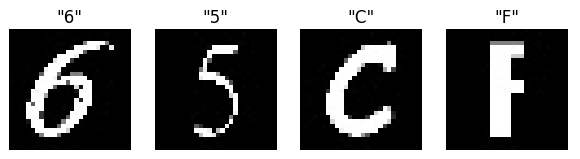
\includegraphics[width=0.9\linewidth]{kennzeichenerkennung/matplotlibbsp.png}
    \caption{Beispiel einer Anwendung von Matplotlib}
\end{figure}

Um Matplotlib zu installieren muss das Folgende in der Konsole eingegeben werden:

\begin{listing}[H]
    \begin{minted}{bash}
    pip install matplotlib
    \end{minted}
    \caption{PIP Installation von Matplotlib}
\end{listing}

\paragraph{Keras}\mbox{}\\
Keras ist eine Deep-Learning Schnittstelle für diverse Machine Learning Frameworks wie zum Beispiel Tensorflow oder Theanos. 
Damit wird die Bedienung und Anwendung dieser Frameworks vereinfacht und es bietet auch diverse Funktionen, um Inputs mit 
den Machine Learning Modellen kompatibel zu machen. Keras ist ein Teil von Tensorflow, wird aber eigenständig weiterentwickelt, 
um die Kompatibilität mit anderen Machine Learning Frameworks aufrechtzuerhalten. In dieser Applikation wird es in 
Zusammenarbeit mit Tensorflow verwendet, um mit den verwendeten Machine Learning Modellen zu arbeiten.\\

Um Keras zu installieren führt man folgenden Befehl in der Konsole aus:

\begin{listing}[H]
    \begin{minted}{bash}
    pip install keras
    \end{minted}
    \caption{PIP Installation von Keras}
\end{listing}

\paragraph{Tensorflow}\mbox{}\\
Tensorflow ist eines der weltweit beliebtesten Frameworks für Machine Learning und wird von weltweit erfolgreichen Firmen wie 
zum Beispiel Google, AMD oder auch Intel verwendet. Es bietet eine umfassende Plattformen für jegliche Machine Learning Anwendungen 
und ist in Zusammenarbeit mit APIs wie zum Beispiel Keras leicht zu verwenden. In dieser Applikation wird damit ein neuronales 
Netz trainiert und mehrere Machine Learning Modelle verwaltet und verwendet.\\

Bei der Installation von Tensorflow muss beachtet werden, dass sich diese von Windows zu Raspbian stark unterscheidet. 
Raspbian unterstützt offiziell die benötigte Version von Tensorflow noch nicht und deswegen muss dieses über ein paar Umwege installiert werden.\\

Windows:\\

Die Installation von Tensorflow unter Windows ist einfach, da man es wie andere Libraries einfach über pip installieren kann.

\begin{listing}[H]
    \begin{minted}{bash}
    pip install tensorflow
    \end{minted}
    \caption{PIP Installation von Tensorflow}
\end{listing}

Raspbian:\\

Bei Raspbian muss Tensorflow manuell kompiliert werden, da die aktuelle Version noch nicht offiziell unterstützt wird. Diese funktioniert 
aber trotz dieses Umweges einwandfrei und wird mit den folgenden Befehlen in der Konsole installiert.\\

Mit dem ersten Befehl werden die benötigten Tools installiert:

\begin{listing}[H]
    \begin{minted}{bash}
    $ sudo apt-get install cmake curl
    \end{minted}
    \caption{Benötigte Tools für Tensorflow}
\end{listing}

Danach kann man die neuste Tensorflow Version von GitHub herunterladen:

\begin{listing}[H]
    \begin{minted}{bash}
    $ wget -O tensorflow.zip https://github.com/tensorflow/tensorflow/archive/v2.4.0.zip
    \end{minted}
    \caption{Tensorflow von GitHub herunterladen}
\end{listing}

Anschließend muss Tensorflow entpackt werden:

\begin{listing}[H]
    \begin{minted}{bash}
    $ unzip tensorflow.zip
    $ mv tensorflow-2.4.0 tensorflow
    $ cd tensorflow
    \end{minted}
    \caption{Entpacken von Tensorflow}
\end{listing}

Im nächsten Schritt müssen noch zusätzlich erforderliche Libraries installiert werden:

\begin{listing}[H]
    \begin{minted}{bash}
    $ ./tensorflow/lite/tools/make/download_dependencies.sh
    \end{minted}
    \caption{Zusätzlich erforderliche Librarys}
\end{listing}

Danach kann die Installation kompiliert werden:

\begin{listing}[H]
    \begin{minted}{bash}
    $ ./tensorflow/lite/tools/make/build_aarch32_lib.sh
    \end{minted}
    \caption{Kompilieren von Tensorflow}
\end{listing}

Danach muss man die Installation mit den folgenden Befehlen abschließen:

\begin{listing}[H]
    \begin{minted}{bash}
    $ cd ~/tensorflow/tensorflow/lite/tools/make/downloads/flatbuffers
    $ mkdir build
    $ cd build
    $ cmake ..
    $ make -j4
    $ sudo make install
    $ sudo ldconfig
    \end{minted}
    \caption{Abschließen der Installation von Tensorflow}
\end{listing}

Nach diesem Schritt sollte Tensorflow Installation funktionieren und man kann es wie jede andere Library in Python einbinden.

\paragraph{localutils}\mbox{}\\
localutils ist ein einfaches Python-Script, welches die Arbeit mit WPOD-NET im Bereich der Kennzeichenerkennung vereinfacht 
und in dieser Applikation für die einfachere Nutzung von WPOD-NET verwendet wird. Es beinhaltet die Funktion „detectlp“ mit 
welcher ein Bild des Kennzeichens und die Koordinaten des Kennzeichens ermittelt werden können. Dieses Script kann über den 
folgenden Link von GitHub heruntergeladen werden: \url{https://github.com/quangnhat185/Plate_detect_and_recognize/blob/master/local_utils.py} 

\paragraph{Scikit-learn}\mbox{}\\
Scikit-learn ist eine freie Library für Machine Learning und basiert auf Numpy und Matplotlib. Es wird vor allem verwendet, 
um mit großen visuellen Datensätzen neuronale Netze zu trainieren.  Es bietet Funktionen, um Modelle anzupassen, Daten vorzubereiten, 
Modelle zu trainieren und ähnliches. In dieser Applikation wird es für die Normalisierung von Labels verwendet, um diese für Machine 
Learning Modelle anzupassen und für das zufällige Aufteilen von Arrays in Test und Trainingsteile, welche für das Training eines Neuronalen Netzes benötigt werden.\\

Für die Installation von Scikit-learn muss die folgende Zeile in der Konsole ausgeführt werden:

\begin{listing}[H]
    \begin{minted}{bash}
    pip install scikit-learn
    \end{minted}
    \caption{PIP Installation von Scikit-learn}
\end{listing}

\paragraph{Requests}\mbox{}\\
Requests ist eine Library mit welcher HTTP-Anfragen in Python vereinfacht werden. Sie wird häufig verwendet, um mit APIs zu kommunizieren 
und ist eine der beliebtesten Python Librarys, da sie für API-Anwendungen so gut wie notwendig ist. In dieser Applikation wird sie für die 
Kommunikation zu einer eigenen API für den Datenbankzugriff verwendet. Dadurch ist es ohne größere Schwierigkeiten möglich, das Bild des Kennzeichens, 
die ID für den jeweiligen Parkplatz und das Resultat des Kennzeichens an die eigene Datenbank zu senden und auch eine Antwort zu erhalten, ob der 
Zugriff erfolgreich war. Um die Daten mit dieser Library zu übertragen müssen diese einfach nur in einem Dictionary eingetragen werden und dann mit 
dem korrekten Schlüsselwort über die API gesendet werden.\\

Die Installation von Requests erfolgt mit folgendem Befehl in der Konsole:

\begin{listing}[H]
    \begin{minted}{bash}
    pip install requests
    \end{minted}
    \caption{PIP Installation von Requests}
\end{listing}

\paragraph{Gpiozero}\mbox{}\\
Gpiozero ist eine Python-Library für den Raspberry Pi. Mit ihr ist es möglich auf die GPIO-Pins des Raspberry zuzugreifen, Signale von diesen 
auszulesen und Signale an diesen auszugeben. Dies wird oft verwendet, um Sensoren auszuwerten oder um Aktoren zu steuern, da diese Pins frei 
programmierbar sind, wodurch man jede beliebige Anwendung realisieren kann. Der Raspberry Pi kann zwar nur Aktoren in seiner Leistungskategorie ansteuern, 
dies kann aber zum Beispiel mit einem Relais umgangen werden, wodurch der Raspberry Pi zu einem mächtigen Werkzeug für die Sensorik und Aktorik wird. 
Ein Beispiel für die möglichen Anwendungen ist ein Button oder eine Lampe. In dieser Applikation wird mit dieser Library ein gedrückter Button detektiert, 
welcher als Auslöser für die Kamera fungiert.\\

In der folgenden Abbildung sieht man ein Bild der GPIO-Pins des Raspberry Pi, welche mit dieser Library angesteuert werden können:

\begin{figure}[H]
    \centering
    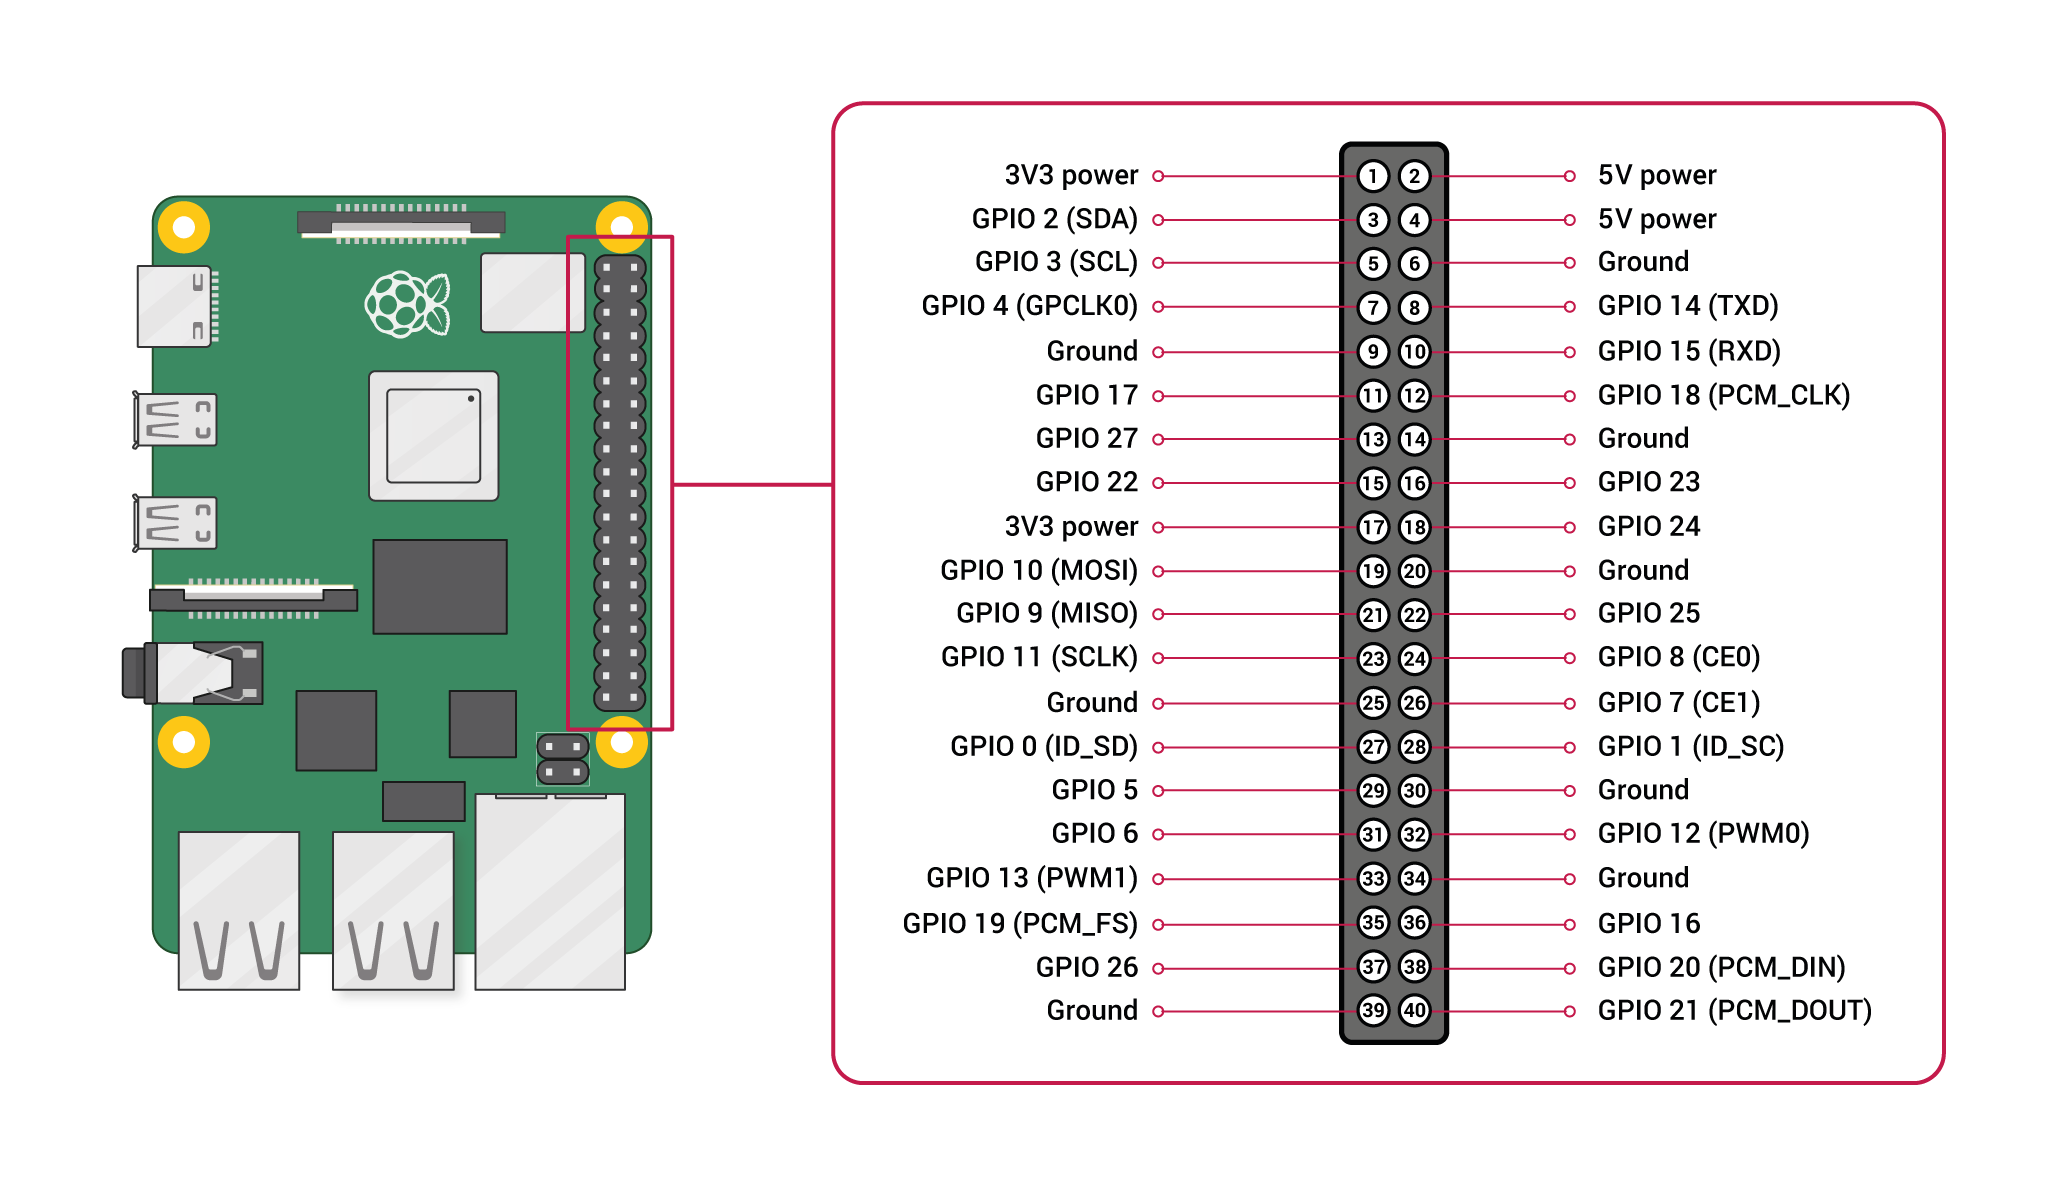
\includegraphics[width=0.8\linewidth]{kennzeichenerkennung/GPIO-Pinout-Diagram-2.png}
    \caption{GPIO-Pins des Raspberry Pi}
\end{figure}

Diese Library kann nur auf dem Raspberry Pi installiert werden. Um die Library Gpiozero zu installieren kann pip verwendet werden:

\begin{listing}[H]
    \begin{minted}{bash}
    pip install gpiozero
    \end{minted}
    \caption{PIP Installation von Gpiozero}
\end{listing}

\paragraph{Picamera}\mbox{}\\
Die Library picamera wird verwendet, um auf das Kameramodul des Raspberry Pi zuzugreifen. Die Library bietet etliche Funktionen an, 
mit welchen die Kamera gesteuert werden kann, wie zum Beispiel Fotos aufzunehmen, Videoaufnahmen zu starten und zu beenden, Fotoeinstellungen 
zu ändern und ähnliches. Die Library ist notwendig, wenn man über Python das Kameramodul bedienen will. In dieser Applikation wird sie verwendet, 
um ein Vorschaubild des aufgenommenen Bildes auf dem Bildschirm darzustellen, falls ein Bildschirm angeschlossen wird und um im 
Anschluss das Bild aufzunehmen und korrekt zu skalieren.\\

Die Installation von picamera ist nur auf dem Raspberry Pi möglich, da nur dieser damit arbeiten kann. 
Für die Installation von picamera muss folgender Befehl in der Konsole eingegeben werden:

\begin{listing}[H]
    \begin{minted}{bash}
    pip install picamera
    \end{minted}
    \caption{PIP Installation von Picamera}
\end{listing}

\subsubsection{Wichtige Programmteile}



\subsection{Raspberry Pi}

\subsubsection{Einleitung}
Damit die Software der Kennzeichenerkennung arbeiten kann, benötigt es eine geeignete Hardware. Diese muss dabei die folgenden Eigenschaften 
aufweisen, um für die Kennzeichenerkennung geeignet zu sein:

\begin{itemize}
    \item Möglichst klein
    \item Nicht zu teuer 
    \item Möglichkeit eine Kamera anzuschließen 
    \item Schnell 
    \item Internetanbindung
\end{itemize}

\subsubsection{Wahl des Raspberry Pi}
In dieser Applikation wird ein RaspberryPi 4B 2GB verwendet, da er alle zuvor genannten Eigenschaften am besten erfüllt.\\

\begin{figure}[H]
    \centering
    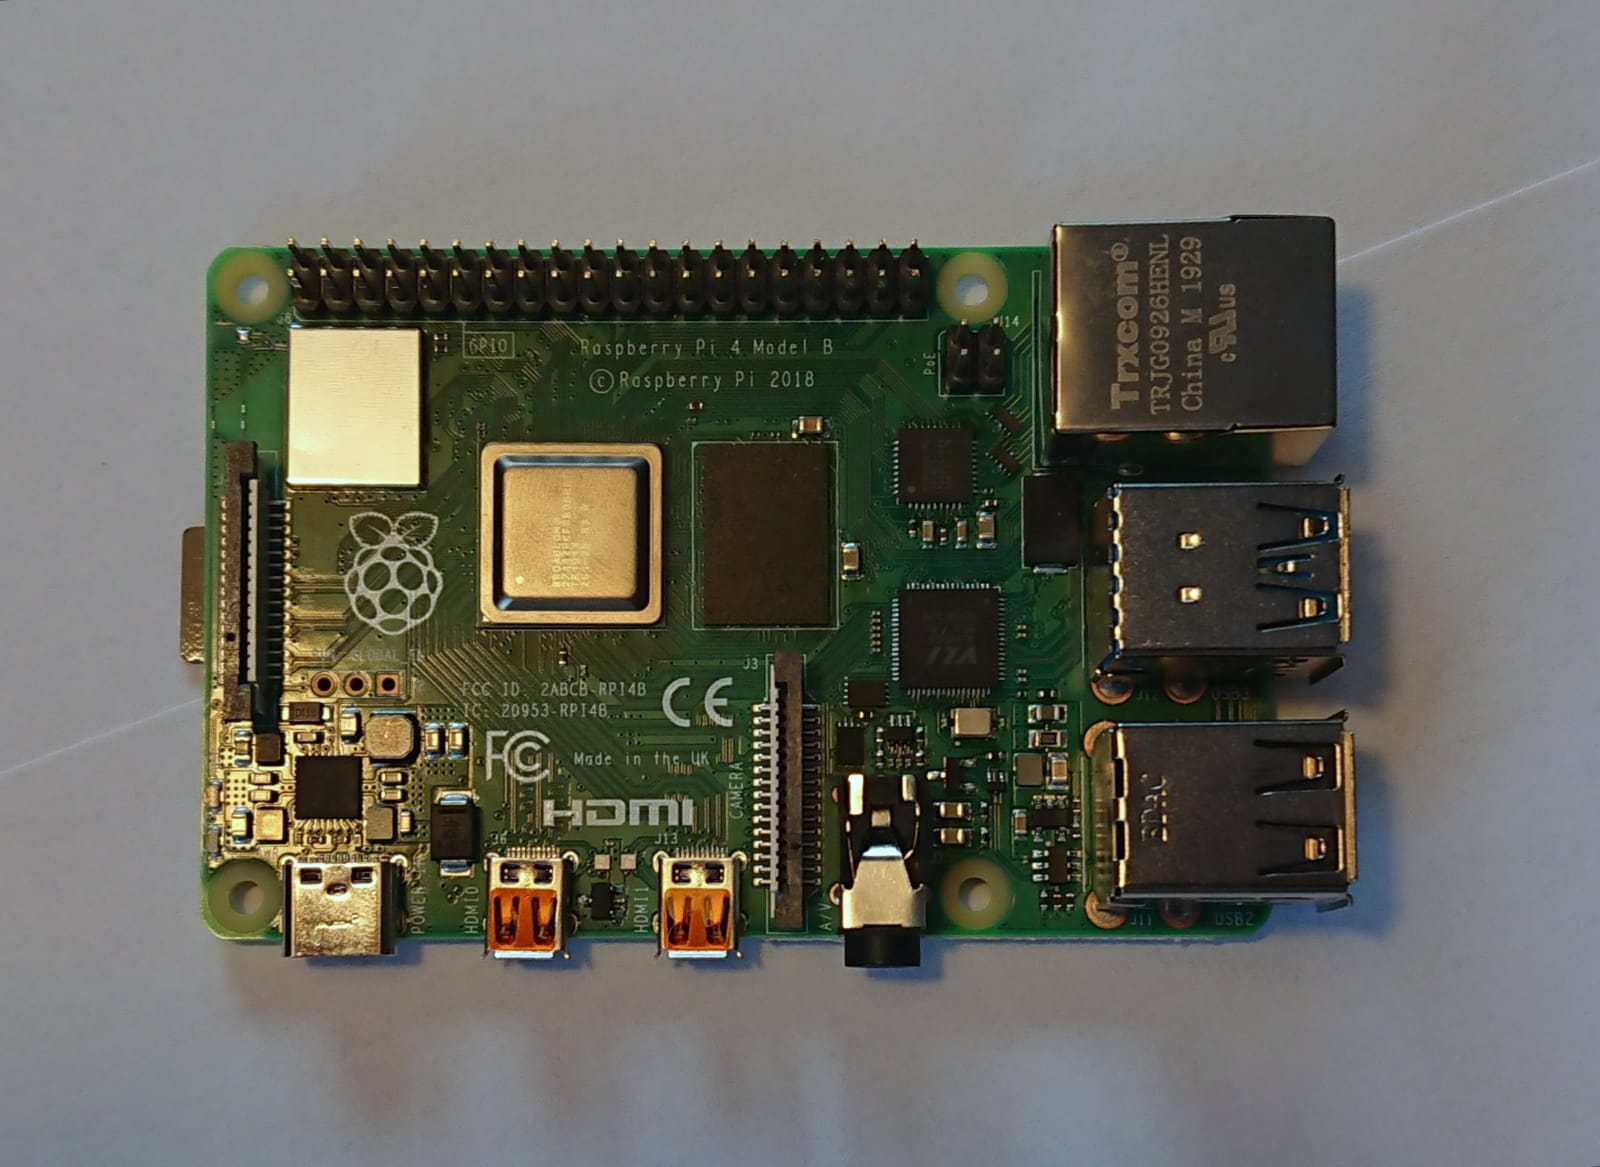
\includegraphics[width=0.6\linewidth]{kennzeichenerkennung/rpi.png}
    \caption{Raspberry Pi}
\end{figure}

Er hat die Größe einer Scheckkarte, wodurch es möglich ist ein kompaktes Gehäuse zu bauen, welches man einfach montieren kann. 
Er ist mit 35€ pro Stück nicht zu teuer. Er hat einen integrierten Kameraanschluss und es gibt unzählige Kameras, welche damit 
kompatibel sind. Er hat für seine Größe eine sehr gute Rechenkraft und ist damit in der Lage das komplette Programm für die 
Kennzeichenerkennung in einer akzeptablen Zeit abzuarbeiten. Er besitzt außerdem einen Ethernet-Anschluss und ein WLAN-Modul, 
wodurch er sehr einfach mit dem Internet verbunden werden kann.

\subsubsection{Kamera}
Für den Raspberry Pi muss zudem noch die passende Kamera ausgewählt werden, um die Bilder von den Kennzeichen aufzunehmen. 
Dafür gibt es Unmengen an kompatiblen Kameras, aber hier wird das Originalzubehör von RaspberryPi verwendet. Dies hat den Grund, 
dass diese Kamera leicht zu verwenden, sehr klein, mit Schrauben einfach zu befestigen und günstig ist. Zudem liefert sie ein 
qualitativ hochwertiges Bild, welches für die Software gut verarbeitbar ist.

\begin{figure}[H]
    \centering
    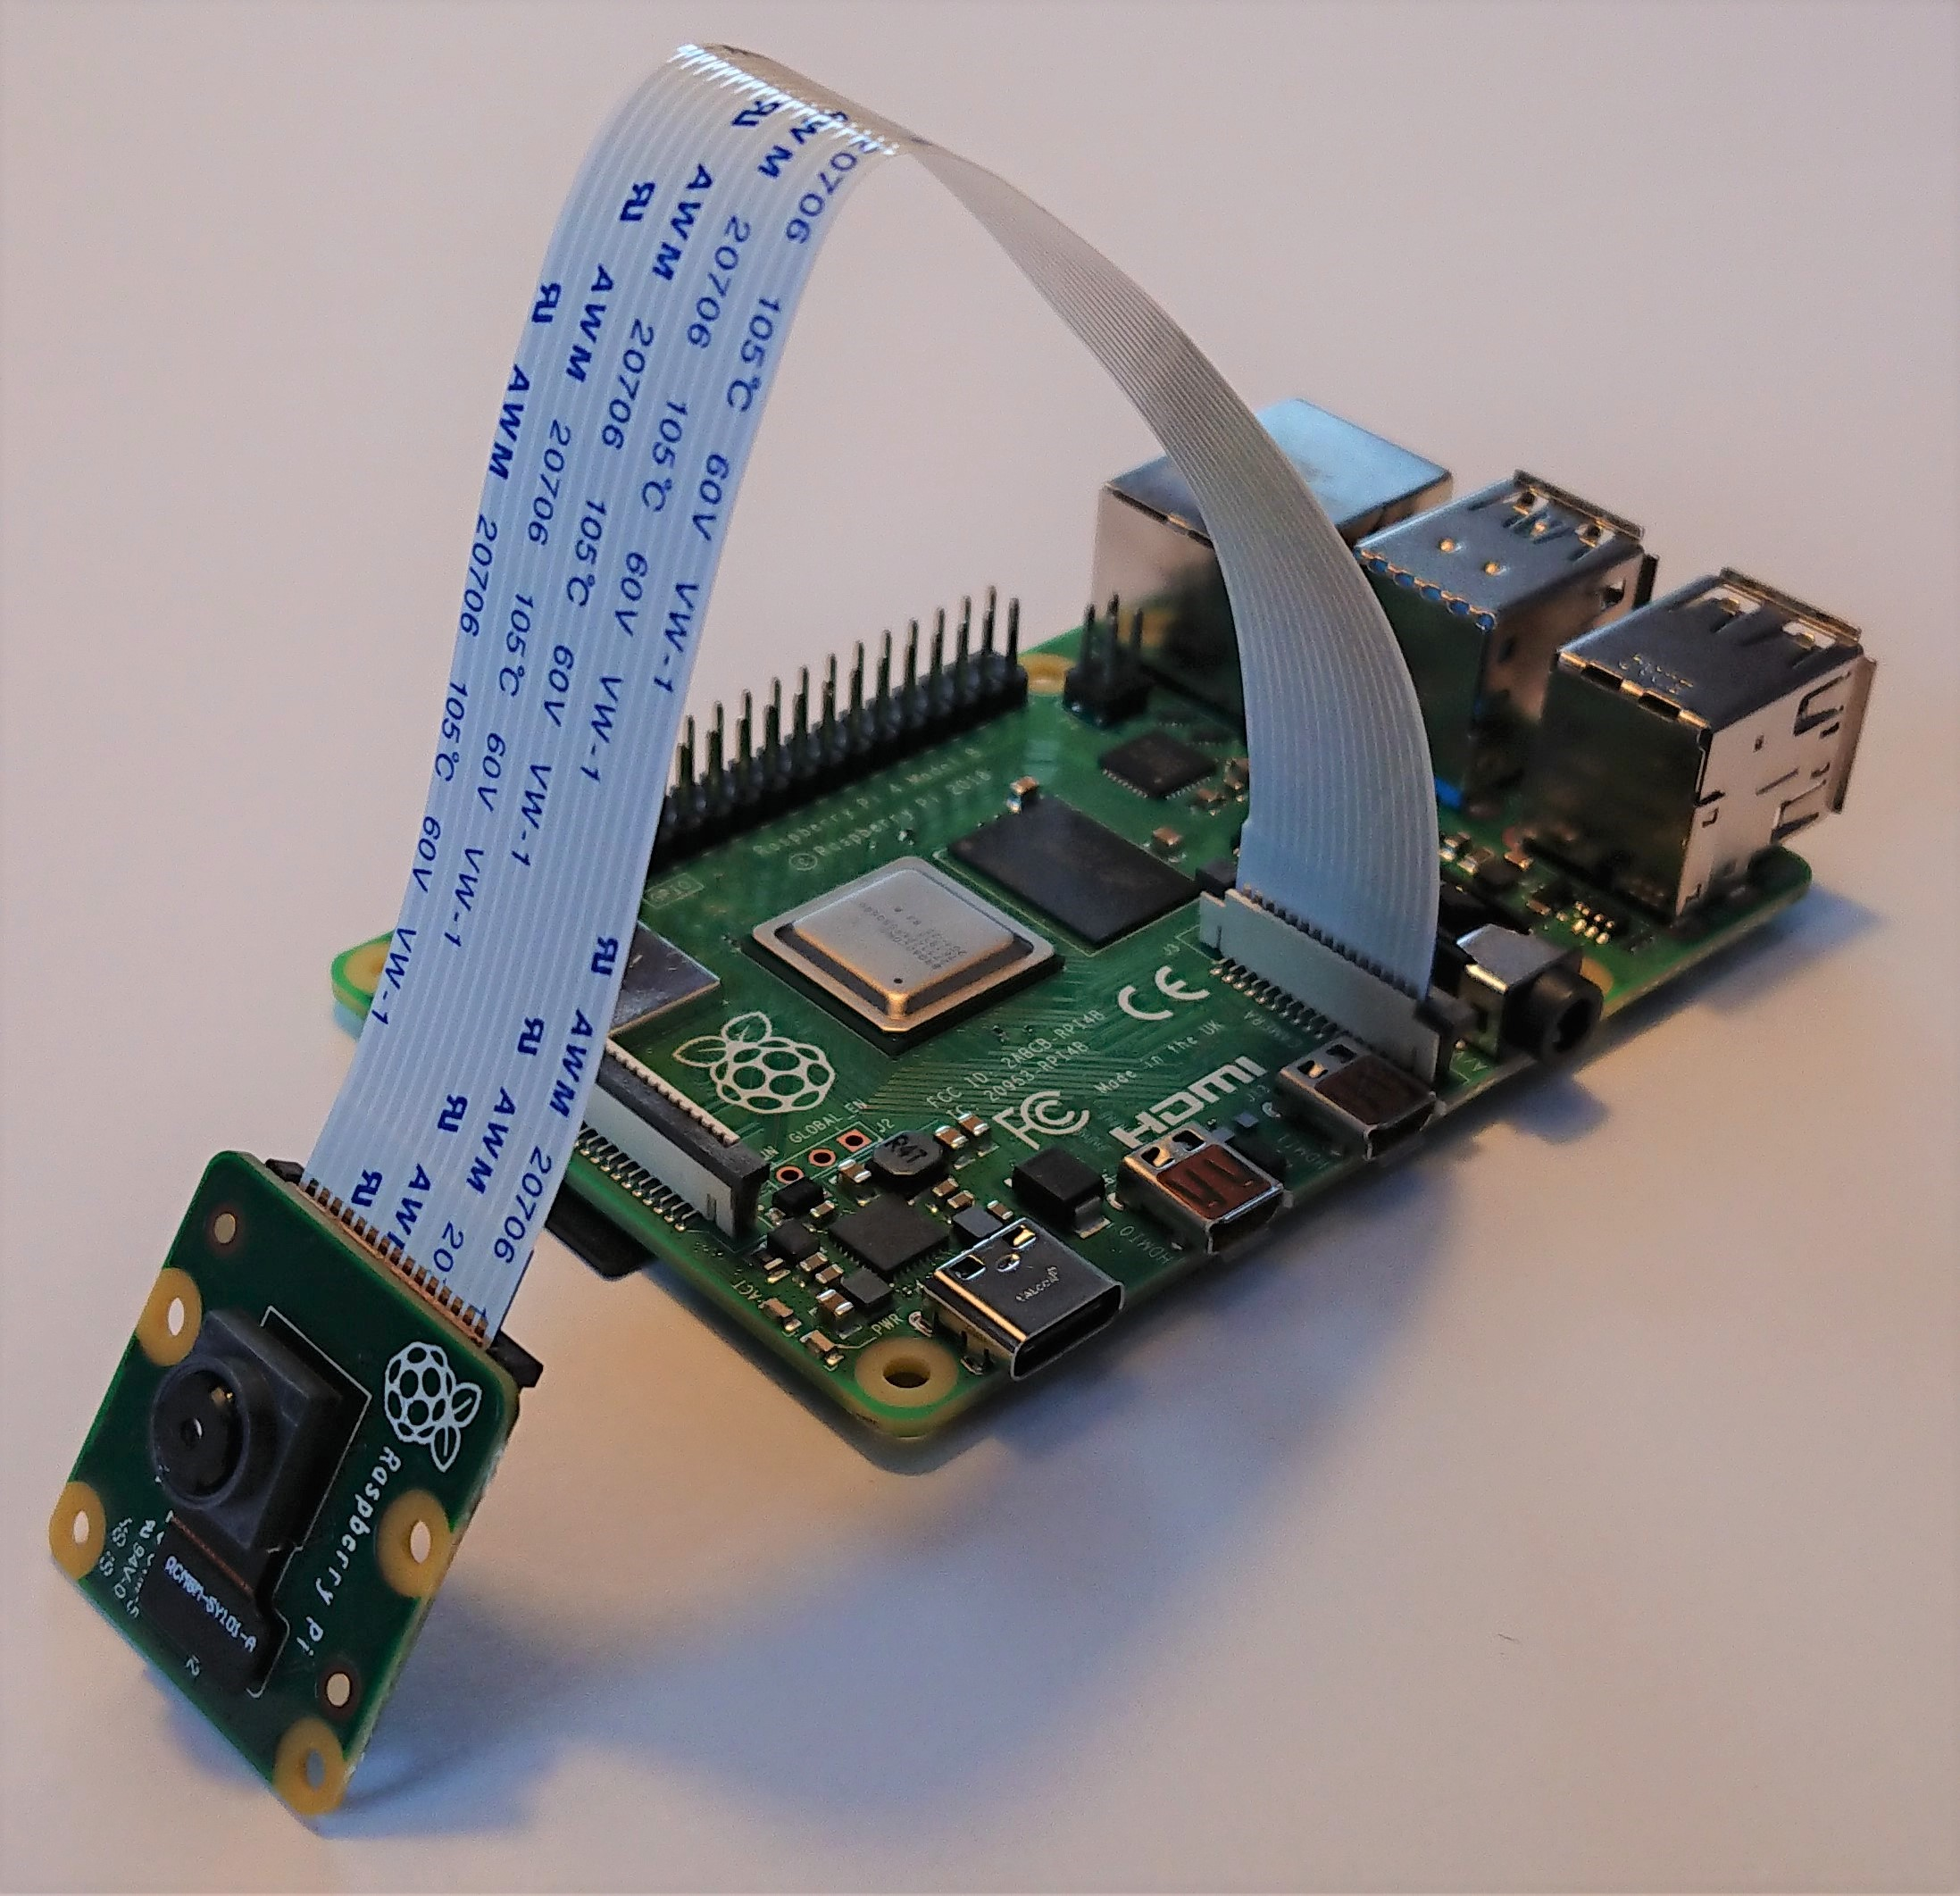
\includegraphics[width=0.6\linewidth]{kennzeichenerkennung/rpiKamera.png}
    \caption{Raspberry Pi mit Kamera}
\end{figure}